\subsection{Discussion}  
We make a number of assumptions and choices in the \eda. For instance, 
\eda~assigns $A_V$ using the slab model (Eq.~\ref{eq:slab}). We use the slab
model because it reproduces the correlation between attenuation and inclination 
in observations~\citep{conroy2010b, wild2011, battisti2017, salim2020} and
simulations~\citep[\eg][]{chevallard2013, narayanan2018, trayford2020}.
It also reproduces the SDSS $A_V$ distribution (Figure~\ref{fig:av_dist}). If
we replace the slab model with a more flexible model for sampling $A_V$ using
truncated normal distributions, we find that our results are not significantly
impacted (see Appendix~\ref{sec:nonslab} for details). Therefore, we conclude
that our results do not sigificantly depend on our choice of the slab model. 

Besides the slab model, we use a simple parameterization of $\tau_V$ and
$\delta$ in the \eda. Both $\tau_V$ and $\delta$ depend linearly on $\log M_*$ 
and $\log {\rm SSFR}$. This linear parameterization was choice for solely for
its simplicity---the \eda~can easily be extended to more flexible
parameterizations. In fact, a more flexible parameterization would likely reduce 
some of the discrepancies with the SDSS color-magnitude relations. The
\eda~produces broader distributions of optical colors than SDSS. Few galaxies
in SDSS have $\gr > 1.$ while some galaxies in the \eda~broadly extend beyond
this cut-off. In the UV, the \eda~struggles to accurately reproduce the redder
portions ($\fnuv > 1.5$) of the UV color-magnitude relation. The main
challenges for a more flexible parameterization would be model selection and
finding a well-motivated parameterization. Nevertheless, for SDSS 
observations, the \eda~using parameter values from the TNG and EAGLE
posteriors find good agreement.

The fact that we can use the \eda~to reproduce SDSS observations for different
hydrodynamical simulations highlights two key points. First, it demonstrates 
that accounting for dust attenuation is essential when comparing simulations to
observations. None of the simulations reproduce the UV and optical
color-magnitude relation without dust attenuation (Figure~\ref{fig:obs}). 
Second, it also highlights the limitations in our current understanding of dust. 
The \eda~is built on our current understanding of dust attenuation in galaxies:
\eg~the \citealt{noll2009} parameterization, the UV bump, the slab model, etc.
Yet with the \eda, two simulations that predict galaxy populations with
significantly different physical properties (Figure~\ref{fig:smf_msfr}) can
reproduce the same SDSS observations. This suggests that dust is highly
degenerate with the differences between simulations. Put another way --- if we 
were to marginalize over dust in our comparison to observations, we would not
be able to differentiate between the different galaxy physics prescriptions in
the simulations. Hence, current limitations in our understanding of dust is 
a major bottleneck for investigating galaxy formation using simulations.


\begin{figure}
\begin{center}
    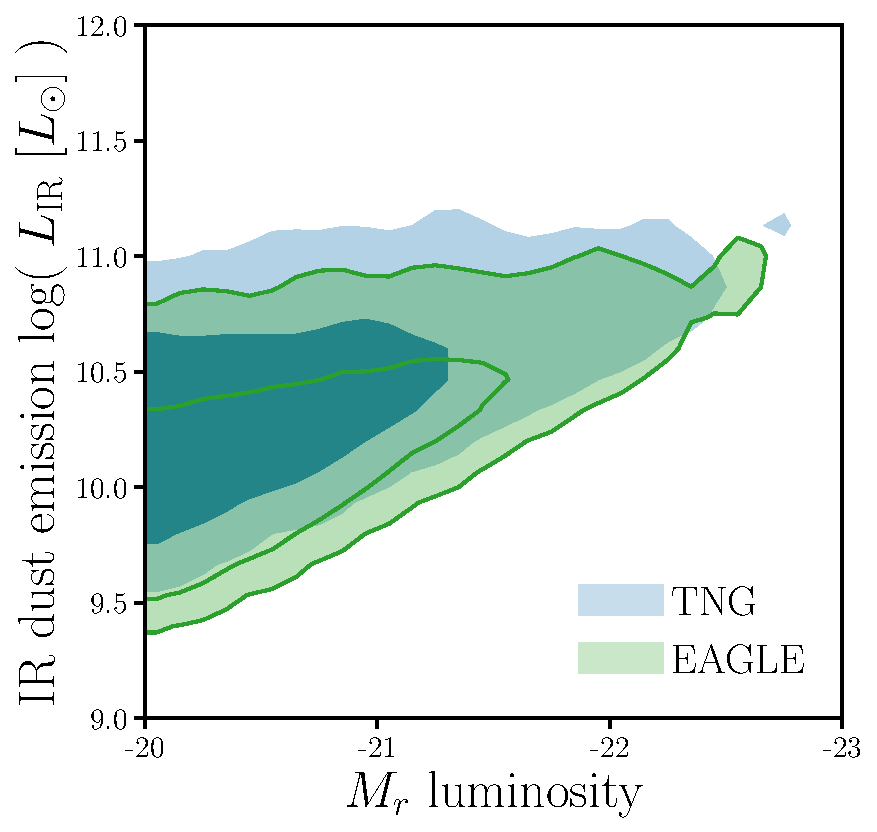
\includegraphics[width=0.45\textwidth]{figs/abc_Lir.pdf}
    \caption{\label{fig:lir}
    IR dust emission luminosity predicted by the \eda~with median parameter
    values of the TNG (blue) and EAGLE (green) posteriors as a function of
    $M_r$. The dust emission is estimated assuming the \cite{dacunha2008}
    energy balance.  Despite reproducing the same SDSS UV and optical
    color-magnitude relations, \emph{the bestfit \eda~models for TNG and EAGLE
    predict significantly different IR dust emission}. Therefore, including IR
    observations will significantly improve the constraints on \eda~parameters
    and allow us to better differentiate galaxy formation models.
    }
\end{center}
\end{figure}

%There's hope! 
Fortunately, there are many avenues for improving our understanding of dust
with a forward modeling approach. In this work, we used a restrictive $M_r <
-20$ complete SDSS galaxy sample. Instead of imposing a completeness limit, 
we can include the actual SDSS selection function in the forward 
model~\citep[\eg~][]{dickey2020}. This would allow us to compare the
simulations with \eda~to a substantially larger galaxy sample. Upcoming
surveys, such as the Bright Galaxy Survey (BGS) of the Dark Energy
Spectroscopic Instrument~\citep[DESI;][]{desicollaboration2016, ruiz-macias2020} 
and galaxy evolution survey of the Prime Focus
Spectrograph~\citep[PFS;][]{takada2014,tamura2016}, will also vastly expand galaxy
observations. BGS, for instance, will measure $10\times$ the number of galaxy
spectra as SDSS out to $z\sim0.4$. A larger more statistically
powerful observation sample will allow us to place tighter constraints on \eda~parameters
and enable an actual comparison of the underlying simulations. 

In this work, we also only used observables derived from UV and optical
photometry. We only examine one side of the impact that dust has on galaxy
spectra. While dust attenuates light in the optical and UV, it emits light in
IR. In fact, even though the TNG and EAGLE simulations reproduce the same UV and
optical color-magnitude relations with the \eda, they predict significnatly 
different dust emission in the IR. In Figure~\ref{fig:lir}, we present IR dust
emission luminosity, $L_{\rm IR}$, predicted by the \eda~with median parameter values of 
the TN (blue) and EAGLE (green) posteriors as as a function of the $r$-band 
absolute magnitude, $M_r$. The dust emissions are estimated using the standard
energy balance assumption --- \ie~all starlight attenuated by dust is reemitted 
in the IR~\citep{dacunha2008}. 

Despite reproducing the same SDSS UV and optical color-magnitude relations, the
bestfit \eda~models for TNG and EAGLE predict significantly different IR dust
emission. The bestfit \eda~model for TNG predicts an overall ${\sim}0.3$ dex
($2\times$) higher dust emissions than for EAGLE. Higher dust emission for TNG
is consistent with the higher $\ctau$ we infer for TNG (Figure~\ref{fig:abc}).
It is also consistent with the fact that TNG predicts bluer galaxies and more
luminous quiescent galaxies with red $\fnuv$ color than EAGLE
(Figure~\ref{fig:obs}). Since IR dust emission measures the total dust
attenuation, IR observations would specifically constrain the \eda~and
therefore break degeneracies between dust and the galaxy physics in simulations.
A number of upcoming observations will probe the IR (\eg~\todo{@tjitske
observations you mentioned}). BGS galaxies will also have IR photometry from
NEOWISE~\citep{meisner2018}. 

% Salim(2020): Chevallard et al. (2013), who aggregated and analyzed a diverse series of theoretical attenuation law studies by Pierini et al. (2004), Tuffs et al. (2004), Silva et al. (1998) and Jonsson et al. (2006), and showed that all the stud- ies predict, with some normalization differences, a relationship between the optical depth AV and attenuation law slope.

% Salmon+(2016): There is evidence that galaxy inclination correlates with the strength of Lyα emission, such that we observe less Lyα equivalent width for more edge-on galaxies (Charlot & Fall 1993; Laursen & Sommer-Larsen 2007; Yajima et al. 2012; Verhamme et al. 2012; U et al. 2015)
% Therefore, based on physi- cal models, one expects that galaxies with “greyer” dust laws and larger overall attenuation should have higher inclinations
% Salim+(2018): Chevallard et al. (2013) furthermore show that the depend- ence of the slope on AV is the same irrespective of whether the AV is driven by different levels of intrinsic (face-on) attenuation or is the result of inclined viewing geometry. 


